\documentclass[11pt,a4paper]{article}
\usepackage{graphicx,psfig,fancyhdr,natbib,subfigure}
\usepackage{epsfig, psfig, epsf}
\usepackage{amsmath, cancel}
\usepackage{amssymb}
%\usepackage{lscape}
\usepackage{dcolumn}% Align table columns on decimal point
\usepackage{bm}% bold math
\usepackage{hyperref,ifthen}
\usepackage{verbatim}



%%%%%%%%%%%%%%%%%%%%%%%%%%%%%%%%%%%%%%%%%%%
%       define Journal abbreviations      %
%%%%%%%%%%%%%%%%%%%%%%%%%%%%%%%%%%%%%%%%%%%
\def\nat{Nat} \def\apjl{ApJ~Lett.} \def\apj{ApJ}
\def\apjs{ApJS} \def\aj{AJ} \def\mnras{MNRAS}
\def\prd{Phys.~Rev.~D} \def\prl{Phys.~Rev.~Lett.}
\def\plb{Phys.~Lett.~B} \def\jhep{JHEP}
\def\npbps{NUC.~Phys.~B~Proc.~Suppl.} \def\prep{Phys.~Rep.}
\def\pasp{PASP} \def\aap{Astron.~\&~Astrophys.} \def\araa{ARA\&A}
\def\jcap{\ref@jnl{J. Cosmology Astropart. Phys.}} 
\def\nar{New~A.R.} 

\newcommand{\preep}[1]{{\tt #1} }

%%%%%%%%%%%%%%%%%%%%%%%%%%%%%%%%%%%%%%%%%%%%%%%%%%%%%
%              define symbols                       %
%%%%%%%%%%%%%%%%%%%%%%%%%%%%%%%%%%%%%%%%%%%%%%%%%%%%%
\def \Mpc {~{\rm Mpc} }
\def \Om {\Omega_0}
\def \Omb {\Omega_{\rm b}}
\def \Omcdm {\Omega_{\rm CDM}}
\def \Omlam {\Omega_{\Lambda}}
\def \Omm {\Omega_{\rm m}}
\def \ho {H_0}
\def \qo {q_0}
\def \lo {\lambda_0}
\def \kms {{\rm ~km~s}^{-1}}
\def \kmsmpc {{\rm ~km~s}^{-1}~{\rm Mpc}^{-1}}
\def \hmpc{~\;h^{-1}~{\rm Mpc}} 
\def \hkpc{\;h^{-1}{\rm kpc}} 
\def \hmpcb{h^{-1}{\rm Mpc}}
\def \dif {{\rm d}}
\def \mlim {m_{\rm l}}
\def \bj {b_{\rm J}}
\def \mb {M_{\rm b_{\rm J}}}
\def \mg {M_{\rm g}}
\def \mi {M_{\rm i}}
\def \qso {_{\rm QSO}}
\def \lrg {_{\rm LRG}}
\def \gal {_{\rm gal}}
\def \xibar {\bar{\xi}}
\def \xis{\xi(s)}
\def \xisp{\xi(\sigma, \pi)}
\def \Xisig{\Xi(\sigma)}
\def \xir{\xi(r)}
\def \max {_{\rm max}}
\def \gsim { \lower .75ex \hbox{$\sim$} \llap{\raise .27ex \hbox{$>$}} }
\def \lsim { \lower .75ex \hbox{$\sim$} \llap{\raise .27ex \hbox{$<$}} }
\def \deg {^{\circ}}
%\def \sqdeg {\rm deg^{-2}}
\def \deltac {\delta_{\rm c}}
\def \mmin {M_{\rm min}}
\def \mbh  {M_{\rm BH}}
\def \mdh  {M_{\rm DH}}
\def \msun {M_{\odot}}
\def \z {_{\rm z}}
\def \edd {_{\rm Edd}}
\def \lin {_{\rm lin}}
\def \nonlin {_{\rm non-lin}}
\def \wrms {\langle w_{\rm z}^2\rangle^{1/2}}
\def \dc {\delta_{\rm c}}
\def \wp {w_{p}(\sigma)}
\def \PwrSp {\mathcal{P}(k)}
\def \DelSq {$\Delta^{2}(k)$}
\def \WMAP {{\it WMAP \,}}
\def \cobe {{\it COBE }}
\def \COBE {{\it COBE \;}}
\def \HST  {{\it HST \,\,}}
\def \Spitzer  {{\it Spitzer \,}}
\def \ATLAS {VST-AA$\Omega$ {\it ATLAS} }
\def \BEST   {{\tt best} }
\def \TARGET {{\tt target} }
\def \TQSO   {{\tt TARGET\_QSO}}
\def \HIZ    {{\tt TARGET\_HIZ}}
\def \FIRST  {{\tt TARGET\_FIRST}}
\def \zc {z_{\rm c}}
\def \zcz {z_{\rm c,0}}


\newcommand{\sqdeg}{deg$^{-2}$}
\newcommand{\lya}{Ly$\alpha$\ }
%\newcommand{\lya}{Ly\,$\alpha$\ }
\newcommand{\lyaf}{Ly\,$\alpha$\ forest}
%\newcommand{\eg}{e.g.~}
%\newcommand{\etal}{et~al.~}
\newcommand{\cii}{C\,{\sc ii}\ }
\newcommand{\ciii}{C\,{\sc iii}]\ }
\newcommand{\civ}{C\,{\sc iv}\ }
\newcommand{\SiIV}{Si\,{\sc iv}\ }
\newcommand{\mgii}{Mg\,{\sc ii}\ }
\newcommand{\feii}{Fe\,{\sc ii}\ }
\newcommand{\feiii}{Fe\,{\sc iii}\ }
\newcommand{\caii}{Ca\,{\sc ii}\ }
\newcommand{\halpha}{H\,$\alpha$\ }
\newcommand{\hbeta}{H\,$\beta$\ }
\newcommand{\oi}{[O\,{\sc i}]\ }
\newcommand{\oii}{[O\,{\sc ii}]\ }
\newcommand{\oiii}{[O\,{\sc iii}]\ }
\newcommand{\heii}{[He\,{\sc ii}]\ }
\newcommand{\nii}{N\,{\sc ii}\ }
\newcommand{\nv}{N\,{\sc v}\ }

%% From:: /cos_pc19a_npr/LaTeX/proposals/JWST/JWST_ERS/Proposal/lines.tex
%%  
\newcommand{\imw}{$i$--$W3$}
\newcommand{\imwf}{$i$--$W4$}
\newcommand{\rmwf}{$r$--$W4$}
\newcommand{\imwt}{$i$--$W2$}
\newcommand{\wtmwf}{$W3$--$W4$}
%\newcommand{\kms}{km s$^{-1}$}
\newcommand{\cmN}{cm$^{-2}$}
\newcommand{\cmn}{cm$^{-3}$}
%\newcommand{\msun}{M$_{\odot}$}
\newcommand{\lsun}{L$_{\odot}$}
\newcommand{\lam}{$\lambda$}
\newcommand{\mum}{$\mu$m}
\newcommand{\ebv}{$E(B$$-$$V)$}
%\newcommand{\heii}{\mbox{He\,{\sc ii}}}
\newcommand{\cv}{\mbox{C\,{\sc v}}}
%\newcommand{\civ}{\mbox{C\,{\sc iv}}}
%\newcommand{\ciii}{\mbox{C\,{\sc iii}}}
%\newcommand{\cii}{\mbox{C\,{\sc ii}}}
%\newcommand{\nv}{\mbox{N\,{\sc v}}}
\newcommand{\niv}{\mbox{N\,{\sc iv}}}
\newcommand{\niii}{\mbox{N\,{\sc iii}}}
%\newcommand{\oi}{\mbox{O\,{\sc i}}}
%\newcommand{\oii}{\mbox{O\,{\sc ii}}}
%\newcommand{\oiii}{\mbox{[O\,{\sc iii}]}}
\newcommand{\oiv}{\mbox{O\,{\sc iv}}}
\newcommand{\ov}{\mbox{O\,{\sc v}}}
\newcommand{\ovi}{\mbox{O\,{\sc vi}}}
\newcommand{\ovii}{\mbox{O\,{\sc vii}}}

%\newcommand{\feii}{\mbox{Fe\,{\sc ii}}}
%\newcommand{\feiii}{\mbox{Fe\,{\sc iii}}}
%\newcommand{\mgii}{\mbox{Mg\,{\sc ii}}}
\newcommand{\neii}{[Ne\,{\sc ii}]\ }
\newcommand{\neiii}{[Ne\,{\sc ii}]\ }
\newcommand{\nev}{Ne\,{\sc v}\ }
\newcommand{\nevi}{[Ne\,{\sc vi}]\ }
\newcommand{\neviii}{\mbox{Ne\,{\sc viii}}}
\newcommand{\aliii}{\mbox{Al\,{\sc iii}}}
\newcommand{\siii}{\mbox{Si\,{\sc ii}}}
\newcommand{\siiii}{\mbox{Si\,{\sc iii}}}
\newcommand{\siiv}{\mbox{Si\,{\sc iv}}}
%\newcommand{\lya}{\mbox{Ly$\alpha$}}
%\newcommand{\lyb}{\mbox{Ly$\beta$}}
\newcommand{\hi}{\mbox{H\,{\sc i}}}
\newcommand{\snine}{\mbox{[S\,{\sc ix}]}}
\newcommand{\sivi}{\mbox{[Si\,{\sc vi}]}}
\newcommand{\sivii}{\mbox[{Si\,{\sc vii}]}}
\newcommand{\siix}{\mbox{[Si\,{\sc ix}]}}
\newcommand{\six}{\mbox{[Si\,{\sc x}]}}
\newcommand{\sixi}{\mbox{[Si\,{\sc xi}]}}
\newcommand{\caviii}{\mbox{[Ca\,{\sc viii}]}}
\newcommand{\arii}{\mbox{[Ar\,{\sc ii}]}}

%%[Ar II] 6.97
%% [S IX] 1.252 μm 328 
% [Si X] 1.430 μm 351 
% [Si XI] 1.932 μm 401 
% [Si VI] 1.962 μm 167 
% [Ca VIII] 2.321 μm 128 
% [Si VII] 2.483 μm 205 
% [Si IX] 3.935 μm 303
% [Ar II] 6.97


%\snine\ at 1.252$\mu$m, \six\ at 1.430$\mu$m, \sixi\ at 1.932$\mu$m, \sivi\ at
%1.962$\mu$m, \caviii\ at 2.321$\mu$m, \sivi\ at 2.483$\mu$m \siix\ at
%3.935$\mu$m and \arii\ at 6.97$\mu$m. 
%%
%% such as [Ne ii]12.8 μm, [Ne v]14.3 μm, [Ne iii]15.5 μm, [S iii]18.7 μm and 33.48 μm, [O iv]25.89 μm and [Si ii]34.8 μm (e.g
%%
%% MIR emission lines like [NeII] and [NeV] are ..
%%
%% Also,  arXiv:astro-ph/0003457v1 
%% [NeV] 14.32um & 24.32um and [NeVI] 7.65um imply an A(V)>160 towards the NLR...
%% [NeIII]15.56um/[NeII]12.81um
%%
%% [Ne V] 14.3, 24.2 μm 97.
%% [Ne II] 12.8 μm
%% [OIV] 26μm
%%


\begin{document}

%% On Aug 10, 2017, at 7:17 PM, Saavik K Ford <sford@amnh.org> wrote:

This is NPRs compilation, and current understanding of, the emails and
discussions that went back in forth first in late July, and then
moreover around the 10th August and the first week in September.

The basic picture is outlined below and given in Figure~\ref{fig:redink}. 

\begin{enumerate}
\item We start with an inflated disk, with non-zero torque at the
ISCO, and $h/R\sim0.2$ inside of $R\sim100 R_{\rm g}$.  This is the
initial state in circa 2000.

\item `Something' happens, around 2007, to provoke a switch to a zero
torque at ISCO state.

There are two basic scenarios to this `something':.  First, this could
is likely due to going from a nonzero torque (NZT) condition at the
inner boundary of the disk to a zero torque (ZT) condition. This could
be triggered by a $B$-field collapse, contraction or ejection close to
the BH.  Alternatively, using the ``Lamppost model'' of AGN coronae,
the lamppost is being raised so there is less heating of the inner
disk and the cooling front propagates outwards.
 
%% So, we could say something like, "changes in the inner disk boundary condition or the corona above the BH, would account for the pattern of observations presented here, and make different (testable) predictions for future behaviour of this source.'

\item A cooling front is set-up, which propagates out from the ISCO at
the timescale, $t_{\rm front}$. Regions behind the front emit flux at
0.1 of what they did prior to the passage of the front (due to drop in
T? T $\downarrow \times 1.78 \Rightarrow L \downarrow \times10$) , and
the temperature decrease leads the height to drop by a factor of 2
(just due to less kinetic energy??).  $L_{\rm ion}$ starts dropping
due to the drop in ionizing photons, which in turn causes the H-lines
to also start to drop.

\item Because the disk starts fat, the cooling front time is not that
long, and by 2010 (3 years later), the front has reached $R\sim50
R_{g}$. During that time, the collapsing disk height increases the
number density of scatterers, which in turn causes Rayleigh scattering
producing the blue downturn in the 2010 spectrum.

\item The cooling front keeps going, until it hits the part of the
disk where it is normally thin, around $R=100 R_g$, arriving around
2012. This sets up another (heating) front, which will travel {\it
back in} towards the SMBH, and re-inflate the disk. This 'returning'
front travels more slowly because the disk is thinner. It also means
the return to normal will be asymmetric in time, as observed, and the
$g$-band bottoms out first because that is coming from
$R\sim100R_{g}$.

\item We expect the front to return to the ISCO in about 2018. That
means the H lines will come back a few months later, but the WISE IR
flux shouldn't come back until about 2021.

\end{enumerate}


\begin{figure*}
  \centering
  %% trim=l b r t 
  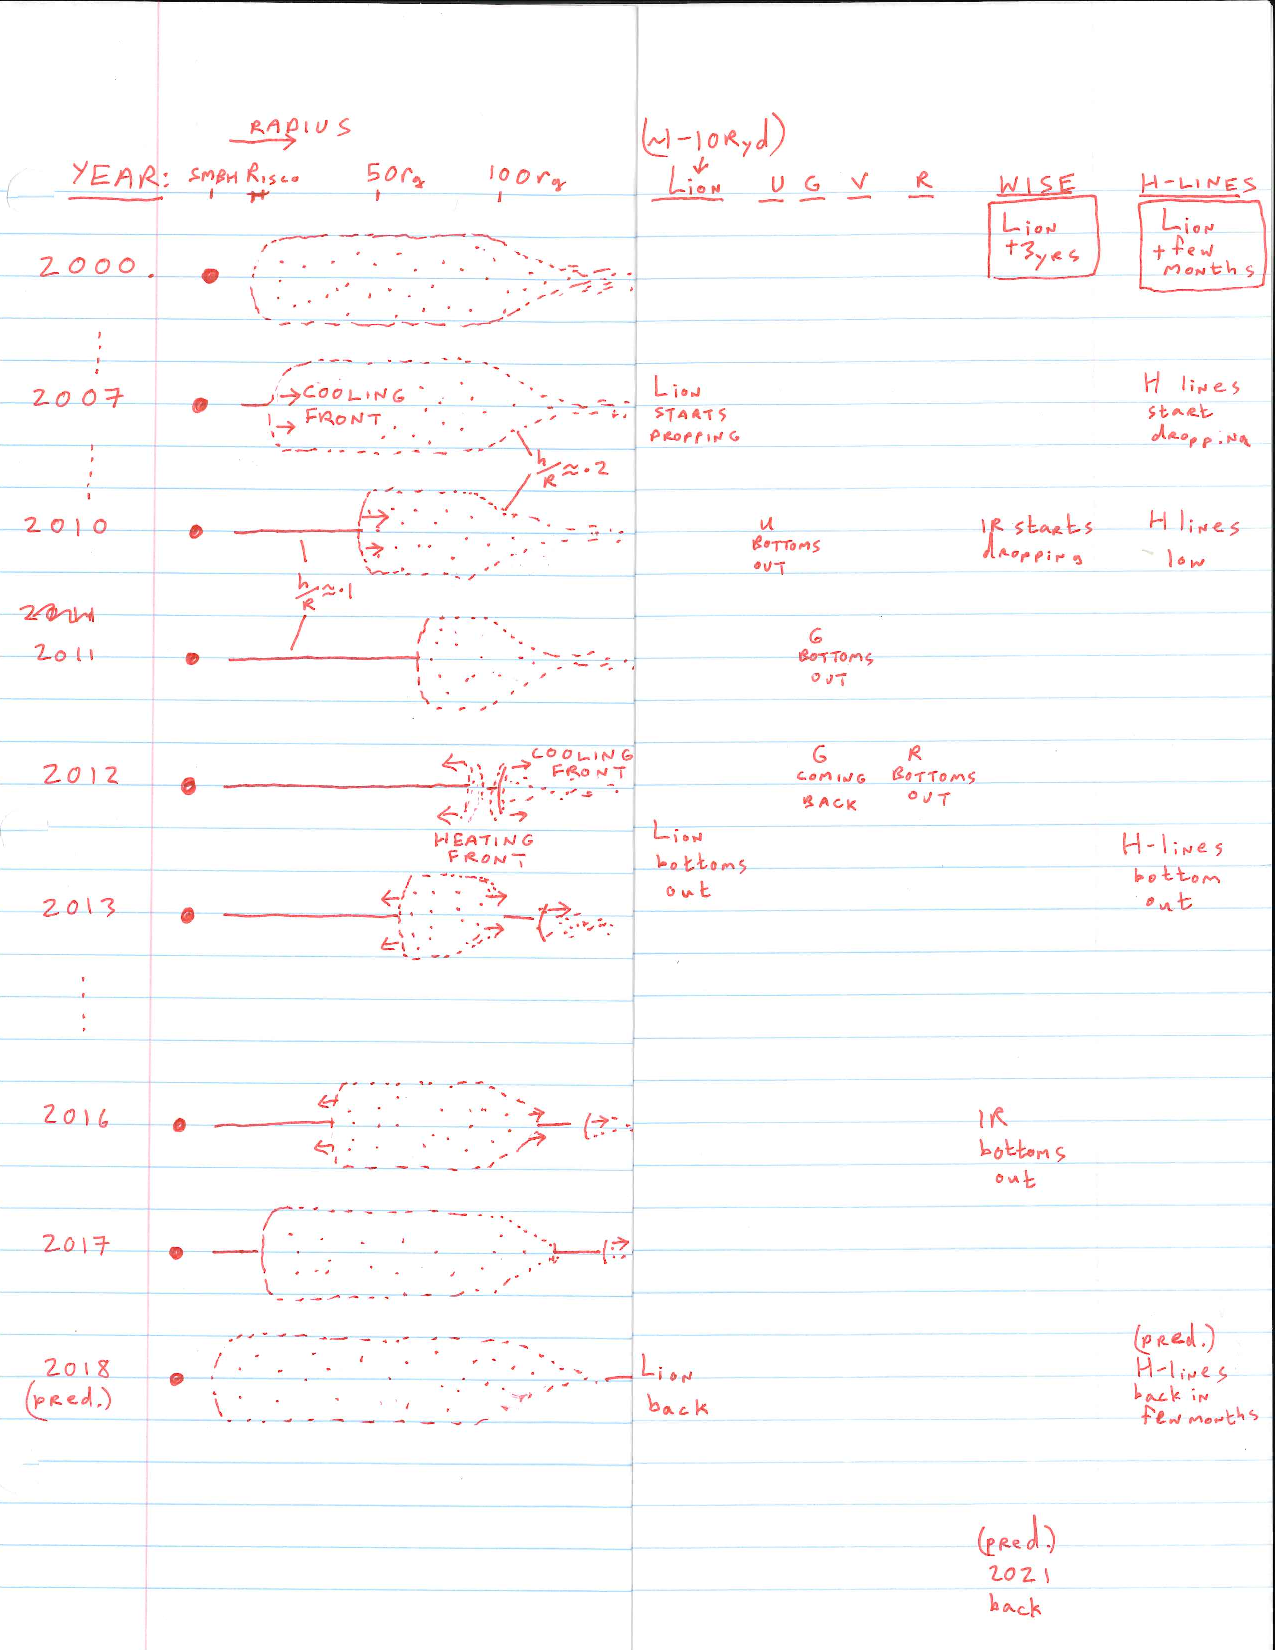
\includegraphics[width=16.00cm, trim=0.0cm 0.0cm 0.0cm 0.0cm, clip] 
  {simple_model.pdf}
  \caption[]{
Our working model explaining the optical and IR light-curves, the
change seen in the 3 spectra, {\it and} making predictions to what
will be seen in 2018 and 2021.
}
  \label{fig:redink}
\end{figure*}



\iffalse
\newpage
\section{Reminder of just some BH Basics ;-)} 

\subsection{Innermost Stable Circular Orbit}
\begin{equation}
g_{\mu \nu} = 
\begin{pmatrix}
(1- \frac{2M}{r})   & 0                                  & 0         & 0  \\ 
0                          & (1- \frac{2M}{r})^{-1}    & 0         & 0 \\ 
0                          & 0                                  & r^{2}   & 0 \\ 
0                          & 0                                  & 0         & r^2 \sin^2\theta\\
\end{pmatrix}
\end{equation}

\begin{equation}
V_{\rm eff}(r) = - \frac{M}{r}  + \frac{l^2}{2r^2} - \frac{Ml^2}{r^3}
\end{equation}
with the first two terms being Newtonian and the third a correction. 

$\Rightarrow$
\begin{equation}
\frac{d V_{\rm eff}}{dr} = - \frac{M}{r^{-2}}  - \frac{l}{r^{3}} - \frac{3 M l^2}{r^{-4}}
\end{equation}
Set to zero, $\Rightarrow$
\begin{equation}
r_{\pm} = \frac{l^2}{2M} \left (1 \mp \sqrt{1 - 12   \frac{M^2}{l^2}     }   \right ).
\end{equation}
I think I've got my $+/-$ signs the right way round, but it's based on the metric definition, 
and not important for the final result, i.e.,  this value is at an extremum when 
\begin{equation}
\frac{l^2}{M^2} = 12.
\end{equation}
(I think there is also some $G=c=1$ going on in the above equations ;-)\\
Thus, $r_{\rm min} = 6 M$, and the corresponding radius for the
{\bf innermost stable circular orbit}, $R_{\rm ISCO}$, is then
\begin{equation}
R_{\rm ISCO} = \frac{6 G M}{c^{2}} = 6 R_{\rm g} =  3 R_{\rm Sch}
\end{equation}
and 
\begin{equation}
R_{\rm Sch} = \frac{2 G M}{c^2}
\end{equation}
and 
\begin{eqnarray}
R_{\rm g}  & = &  \frac{G M}{c^2} \\
                 & = &   1.4822 \left ( \frac{M}{M_{\odot}} \right ) {\rm km}\\
              & = & M_{8} {\rm AU}\\
\end{eqnarray}
where $M_{8} = 1.00 \times10^{8} M_{\odot}$ (to within $\approx1.5\%$)
i.e. the gravitational radius of a 1e8 $M_{\rm solar}$ black hole is 1
AU.  I am trying to use captial $R$ for the `named' radii; the
gravitational radius can be capital or lowercase.

\subsection{Accretion disk temperature}
%Looking at \citet{Zimmerman05} in particular.
{\bf Looking at Zimmerman et al. (2005) in particular.}
Fitting spectra with the multitemperature blackbody (MTB) model allows
us to determine important properties of accretion disks, including
accretion rate, inner radius, and temperature
%\begin{equation}
%\end{equation}
Over the years, a number of different assumptions have been used in
deriving the MTB spectrum. A standard assumption in the literature is
that a zero-torque boundary condition should be applied to the inner
edge of the accretion disk (Shakura \& Sunyaev 1973; Novikov \& Thorne
1973).


``Ideas about discs nevertheless gained credibility because of two
factors. The first was that the radial distribution of effective
temperature across a steady disc $[ T (R) \propto R^{-3/4} ]$ is
independent of the viscosity, being just a statement of energy
conservation, and is in reasonable accord with both continuum spectra
and eclipse mapping of cataclysmic variables (CVs).'' -- (think this
is from an Andrew King paper introduction)

\fi




\end{document}
